\subsection{Dispositivo}

En cuanto a la arquitectura final del dispositivo, no va a ser especificada ya que el presente proyecto no se adentra en la implementación del asistente, sino que pone las pautas y los protocolos mediante los cuales el asistente podrá comunicarse con el servidor.

Para poder mostrar estas pautas se ha implementado un controlador de pruebas, que será explicado junto a los casos de uso del dispositivo, pudiendo permitir posteriormente el desarrollo del asistente virtual inteligente con cualquiera de los métodos existentes.

\subsection{BackEnd} \label{arch-be}

Como se ha nombrado anteriormente, el sistema desarrollado en la parte del servidor deberá servir una API REST, de modo que la arquitectura elegida para la implementación del backend es una arquitectura REST, la cual se basa en ofrecer unos end-points desde los cuales se trata la información almacenada en el sistema.

Para una mejor implementación de esta arquitectura, se estructura el sistema bajo la Clean Architecture, de modo que se permite el desarrollo del sistema en una organización formada por capas, donde el acceso a la siguiente capa es lineal, evitando dependencias cruzadas que perjudiquen la escalabilidad del sistema.

\begin{figure}[h!]
    \centering
    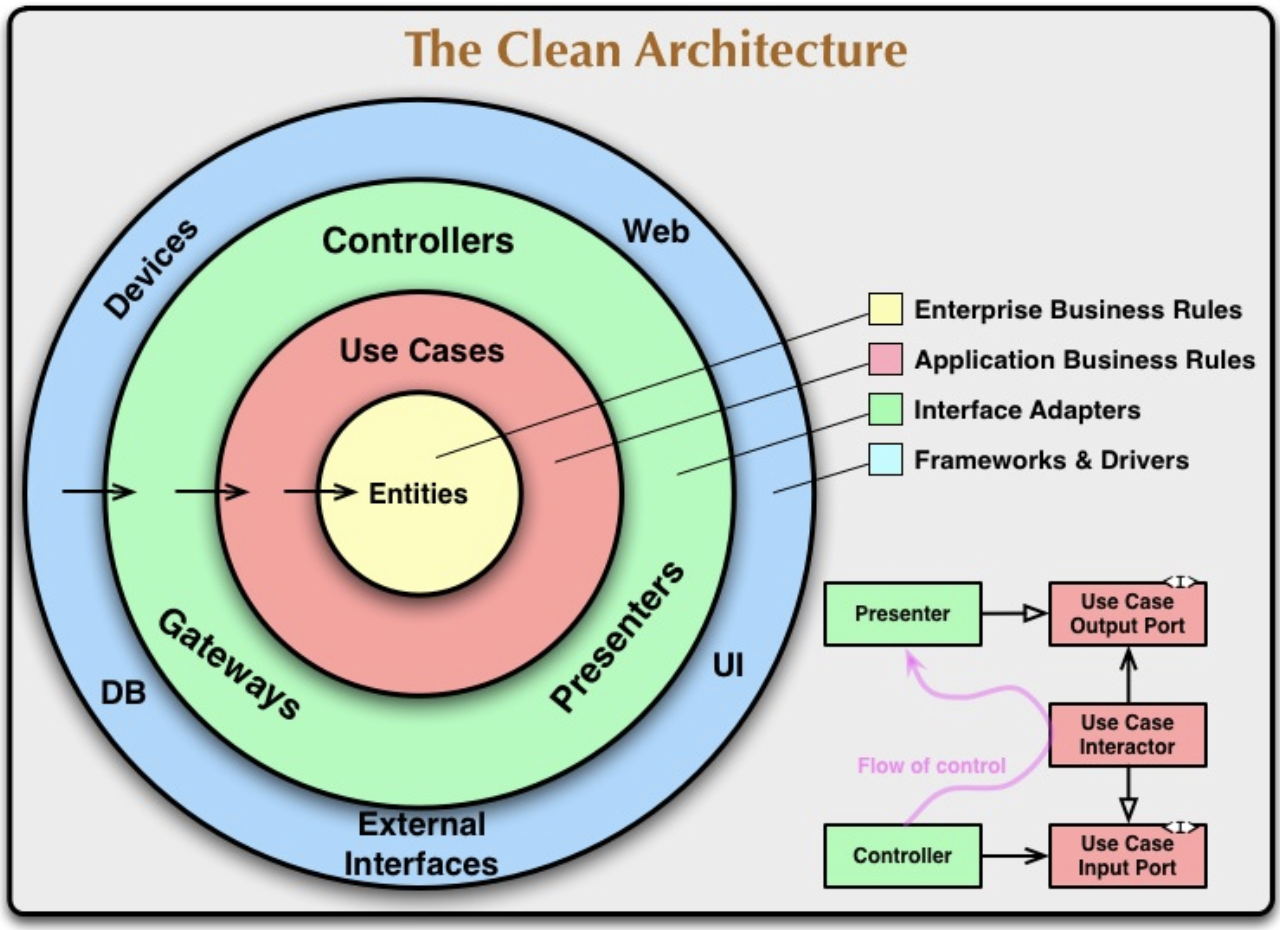
\includegraphics[width=7cm]{./img/arch/cleanarch.png}
    \caption{The Clean Architecture}
    \label{fig:cleanarch}
\end{figure}

\subsection{FrontEnd}

El sitio web a desarrollar para la administración del sistema se contruye a partir del framework javascript de VueJS, como ya se ha mencionado anteriormente en el apartado \ref{Vue}.

VueJS propone una arquitectura MVVM~\cite{mvvm}, en la cual el diseño del sistema se basa en el desarrollo de múltiples componentes: Un componente es una unidad que dispone de su propio sistema de vista-presentador, teniendo una interfaz gráfica implementada en HTML + CSS, que efectúa un comportamiento a través de funciones JavaScript.

Esta modularidad interna basada en componentes debe seguir unas pautas~\cite{vuecomp} para sacar el máximo rendimiento de estos, al igual que para poder en un futuro remplazar o eliminar los componentes creados por otros que se ajusten a los nuevos requisitos sin perjudicar el resto de ellos.

Los datos que se manejan en la web aparecen en la vista de forma dinámica, de manera que es el presentador quien los puede variar.
